% Weekly supervisor update slide deck (Beamer)
% Compile (example): pdflatex weekly_update_ecg200_2026-04-17.tex

\documentclass[aspectratio=169]{beamer}

\usetheme{Madrid}
\usecolortheme{default}

\usepackage{amsmath}
\usepackage{booktabs}
\usepackage{graphicx}
\usepackage{tikz}
\usetikzlibrary{positioning,arrows.meta,fit}
\usepackage{listings}

\title[Weekly update]{Weekly progress update: Explainable clustering workflow (ECG200)}
\subtitle{KMeans + surrogate rules + SHAP (raw vs shapelet-distance features)}
\author{\textit{(your name)}}
\institute{M2 Internship (LIRMM) — Explainable clustering}
\date{17 Apr 2026}

\begin{document}

\begin{frame}
  \titlepage
\end{frame}

\begin{frame}{This week: what I delivered}
  \begin{block}{Outcome}
    End-to-end \textbf{explainable clustering} workflow on ECG200 to validate the approach before porting to picoclimate windows.
  \end{block}
  \vspace{0.4em}
  \begin{itemize}
    \item Two representations: \textbf{raw time points} vs \textbf{shapelet-distance features}
    \item Unsupervised $k$ selection: internal metrics + multi-seed stability
    \item Explanations: surrogate decision tree rules + SHAP attributions
  \end{itemize}
\end{frame}

\begin{frame}{Suggested workflow}
  \centering
  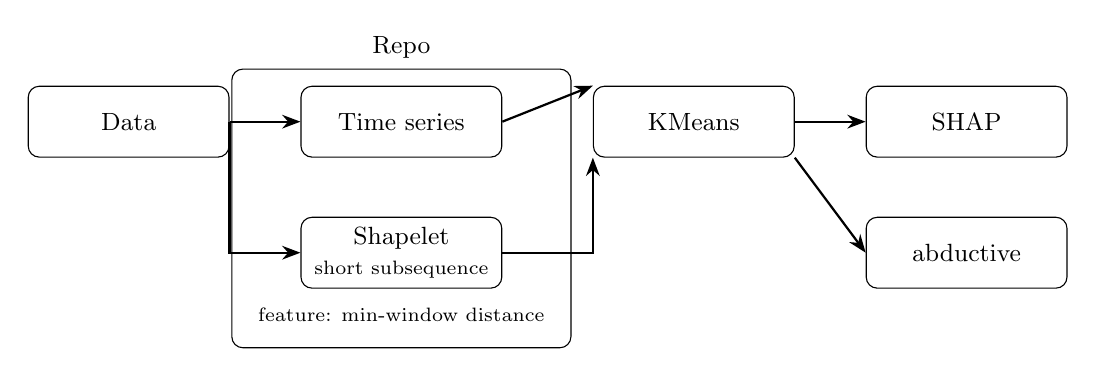
\begin{tikzpicture}[
    node distance=0.75cm and 0.9cm,
    every node/.style={font=\small},
    box/.style={draw, rounded corners, align=center, minimum width=2.55cm, minimum height=0.90cm},
    arr/.style={-{Stealth}, thick}
  ]
    \node[box] (data2) {Data};

    \node[box, right=of data2] (ts) {Time series};
    \node[box, below=of ts] (shapelet) {Shapelet\\{\scriptsize short subsequence}};
    \node[below=0.12cm of shapelet, font=\scriptsize, align=center] (shapelet_note) {feature: min-window distance};

    % Repo grouping around TS + Shapelet (as in the sketch)
    \node[draw, rounded corners, inner sep=6pt, fit=(ts)(shapelet)(shapelet_note), label=above:{\small Repo}] (repo) {};

    \node[box, right=1.15cm of ts] (kmeans2) {KMeans};
    \node[box, right=of kmeans2] (shap2) {SHAP};
    \node[box, below=of shap2] (prod2) {abductive};

    \draw[arr] (data2.east) -- (ts.west);
    \draw[arr] (data2.east) |- (shapelet.west);

    \draw[arr] (ts.east) -- (kmeans2.north west);
    \draw[arr] (shapelet.east) -| (kmeans2.south west);

    \draw[arr] (kmeans2.east) -- (shap2.west);
    \draw[arr] (kmeans2.south east) -- (prod2.west);
  \end{tikzpicture}

  \vspace{0.6em}
  \footnotesize (Clean re-draw of the original hand sketch)
\end{frame}

\begin{frame}{Implemented workflow (high-level)}
  \centering
  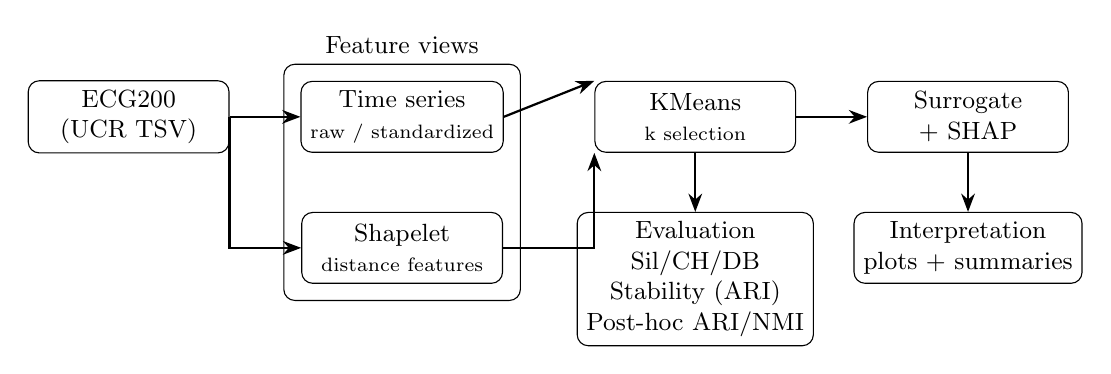
\begin{tikzpicture}[
    node distance=0.75cm and 0.9cm,
    every node/.style={font=\small},
    box/.style={draw, rounded corners, align=center, minimum width=2.55cm, minimum height=0.90cm},
    arr/.style={-{Stealth}, thick}
  ]
    \node[box] (data) {ECG200\\(UCR TSV)};

    \node[box, right=of data] (ts3) {Time series\\{\scriptsize raw / standardized}};
    \node[box, below=of ts3] (shape3) {Shapelet\\{\scriptsize distance features}};
    \node[draw, rounded corners, inner sep=6pt, fit=(ts3)(shape3), label=above:{\small Feature views}] (views3) {};

    \node[box, right=1.15cm of ts3] (kmeans) {KMeans\\{\scriptsize k selection}};
    \node[box, right=of kmeans] (xai) {Surrogate\\+ SHAP};

    \node[box, below=of kmeans] (eval) {Evaluation\\Sil/CH/DB\\Stability (ARI)\\Post-hoc ARI/NMI};
    \node[box, below=of xai] (interp) {Interpretation\\plots + summaries};

    \draw[arr] (data.east) -- (ts3.west);
    \draw[arr] (data.east) |- (shape3.west);
    \draw[arr] (ts3.east) -- (kmeans.north west);
    \draw[arr] (shape3.east) -| (kmeans.south west);

    \draw[arr] (kmeans.east) -- (xai.west);
    \draw[arr] (kmeans.south) -- (eval.north);
    \draw[arr] (xai.south) -- (interp.north);
  \end{tikzpicture}

  \vspace{0.6em}
  \footnotesize Notebooks: \texttt{kmeans\_ecg200.ipynb} and \texttt{kmeans\_ecg200\_shapelets.ipynb}
\end{frame}

\begin{frame}{Representation comparison (why two notebooks)}
  \begin{columns}[T,onlytextwidth]
    \column{0.49\textwidth}
    \begin{block}{A) Raw time points (96 dims)}
      \begin{itemize}
        \item Input: $x \in \mathbb{R}^{96}$
        \item Clustering geometry: Euclidean (raw / standardized)
        \item Explanations: important time indices $t_i$
      \end{itemize}
    \end{block}

    \column{0.49\textwidth}
    \begin{block}{B) Shapelet-distance features ($m$ dims)}
      \vspace{-0.4em}
      \[
        d(x, s)=\min_{t} \lVert x[t:t+L]-s\rVert_2
      \]
      \vspace{-0.9em}
      \begin{itemize}
        \item Input: $[d(x,s_1),\ldots,d(x,s_m)]$
        \item Optional: window z-normalization
        \item Explanations: \emph{pattern present} (distance small)
      \end{itemize}
    \end{block}
  \end{columns}
\end{frame}

\begin{frame}{Unsupervised selection + evaluation (what is reported)}
  \begin{columns}[T,onlytextwidth]
    \column{0.54\textwidth}
    \begin{block}{Unsupervised $k$ choice (no labels)}
      \begin{itemize}
        \item Internal: Silhouette, Calinski--Harabasz, Davies--Bouldin
        \item Stability: 5 seeds \textrightarrow pairwise ARI between runs
        \item Selection: rank-sum (+ small penalty for large $k$)
      \end{itemize}
    \end{block}

    \column{0.44\textwidth}
    \begin{block}{Post-hoc (labels only for eval)}
      \begin{itemize}
        \item ARI / NMI
        \item majority-mapped accuracy
      \end{itemize}
    \end{block}
  \end{columns}

  \vspace{0.3em}
  \footnotesize\textbf{Note:} saved notebook output shows a representative selection \texttt{k=3} for the raw-view run.
\end{frame}

\begin{frame}{Explainability outputs (what supervisors can inspect)}
  \begin{columns}[T,onlytextwidth]
    \column{0.56\textwidth}
    \begin{block}{Surrogate + SHAP}
      \begin{itemize}
        \item Train shallow decision tree to predict \textbf{cluster ID}
        \item Report fidelity: train + 5-fold CV accuracy
        \item SHAP (TreeExplainer): global feature importance + summary plot
      \end{itemize}
    \end{block}

    \column{0.42\textwidth}
    \begin{block}{Cluster interpretation}
      \begin{itemize}
        \item Raw view: time-index features $t_i$
        \item Shapelet view: top shapelets per cluster
        \item Functional boxplots (cluster curve summaries)
      \end{itemize}
    \end{block}
  \end{columns}
\end{frame}

\begin{frame}{Key takeaways (so far)}
  \begin{itemize}
    \item Workflow implemented end-to-end in both representations (raw and shapelet-distance).
    \item Shapelets shift explanations from pointwise ($t_i$) to \textbf{pattern-level} ("subsequence appears").
    \item Multi-seed stability highlights fragile solutions better than single-run metrics.
  \end{itemize}
\end{frame}

\begin{frame}{Next steps + questions (for today’s meeting)}
  \textbf{Next (1 week)}
  \begin{itemize}
    \item Export results (tables/metrics) to CSV/JSON for reproducibility.
    \item Produce protocol-style per-cluster summaries (fixed template) + explanation stability.
    \item Port the pipeline from ECG200 to \textbf{picoclimate window features}.
  \end{itemize}

  \vspace{0.8em}
  \textbf{Questions for supervisors}
  \begin{itemize}
    \item In ECG200 there are 2 true labels, but internal metrics can select $k\neq 2$ and clusters may not align with labels. Is that acceptable (goal = discover structure), or should we \textbf{fix $k$ to \#classes} for this sanity check?
    \item When we move to picoclimate windows (no ground truth), should we prefer \textbf{internal+stability selection of $k$} or a \textbf{domain-chosen $k$} for interpretability/comparison?
  \end{itemize}
\end{frame}

\end{document}
